\documentclass[../DC2019003Bouma.tex]{subfiles}
\begin{document}
\graphicspath{{04_Validation/img/}}
\renewcommand{\chaptermark}[1]{\markboth{\thechapter.\ #1}{}}
\renewcommand{\sectionmark}[1]{\markright{#1}{}}
\pagestyle{fancyreport}
\cleartooddpage
\pagestyle{fancyreport}
\chapter{Numerical Validation}\label{ch:vali}
To numerically validate the theory presented in this work, some first steps are taken in creating a trajectory tracking simulation for mechanical systems with unilateral constraints and spatial friction. This chapter presents an example of such a system tracking a trajectory with simultaneous impacts. While progress is made in creating the numerical validation, the reader should be aware that it is not yet complete. More work is required to validate the LTTHS and PTTHS presented in Chapter~\ref{ch:order} and Chapter~\ref{ch:simult}, respectively, in the sense that the example discussed in this chapter does not yet contain state-and-input-dependent guards, but merely state-dependent guards. First an example system is given in Section~\ref{sec:5sys}, which describes the kinematics and dynamics of an RRR-robot opening a door. Then, the tracking behavior of that system is simulated and presented. Finally, the steps required to complete the numerical validation of the LTTHS/PTTHS associated with the NISTHS are discussed. The chapter is concluded by summary.

\section{A planar 4-DOF system: RRR-robot opening a door}\label{sec:5sys}
In this section, an example of a mechanical system with unilateral constraints is presented, which will be simulated to validate the theory presented in this work. The system is a robot arm with three revolute joints opening a door, in a planar setting. The forward kinematics and equations of motion for that system will be presented in a concise manner. For a more thorough derivation of the equations of motion, the reader is referred to \cite{Rijnen2018b}. 

\subsection{Forward kinematics}\label{sec:5kin}
Let us now consider the system in Figure~\ref{fig:5system1}. The robot consists of four links, where link 0 is connected to the fixed world and link 3 is a foot-shaped end effector. Link 4 is a door connected to the fixed world with a torsional spring and damper. Coordinate frames are attached to each link, which are referred to as $\Psi_0$ to $\Psi_4$. The centers of mass of the links are assumed to be halfway the link, except for the center of mass of link 3. A closer look at link 3 can be seen in Figure~\ref{fig:5system2}, where the parameters $c_{3,x}$ and $c_{3,y}$ position the center of mass of link 3. Also, two additional coordinate frames $\Psi_{3a}$ and $\Psi_{3b}$ are depicted, which are attached to the contact points defined in the end effector for contact modeling. The set of contact points is given by $\mathcal{I} = \{1,2\}$, where contact point 1 and 2 are related to coordinate frames $\Psi_{3a}$ and $\Psi_{3b}$ respectively. The set of guard identifiers, which is written in binary form, is given by $\eta = \{01,10\}$, where $\gamma_{01}$ is related to contact point 1 and $\gamma^{10}$ to contact point 2. in The system is modeled without friction and trajectories with releasing motions are not considered. Therefore, the system does not contain input-dependent guard functions.

\nomenclature[G23]{$\Psi$}{A coordinate frame}%
\nomenclature[RH]{$\Hb^a_b$}{The homogeneous transformation matrix relating frame $\Psi_b$ to $\Psi_a$}%
\begin{figure}[bt!]
\centering
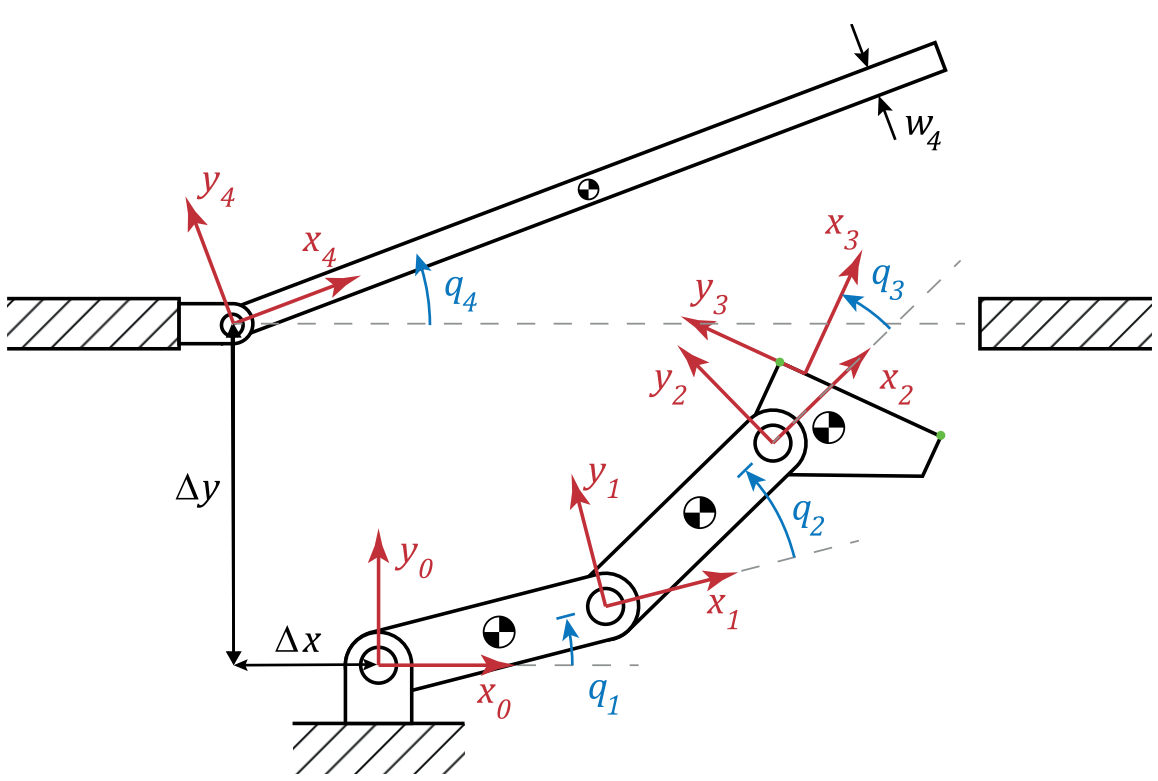
\includegraphics[width=.7\textwidth]{system.PNG}\caption{An RRR-robot and a door in top-down view. This 4-DOF planar system is used to numerically validate the theory presented in this work.}\label{fig:5system1}
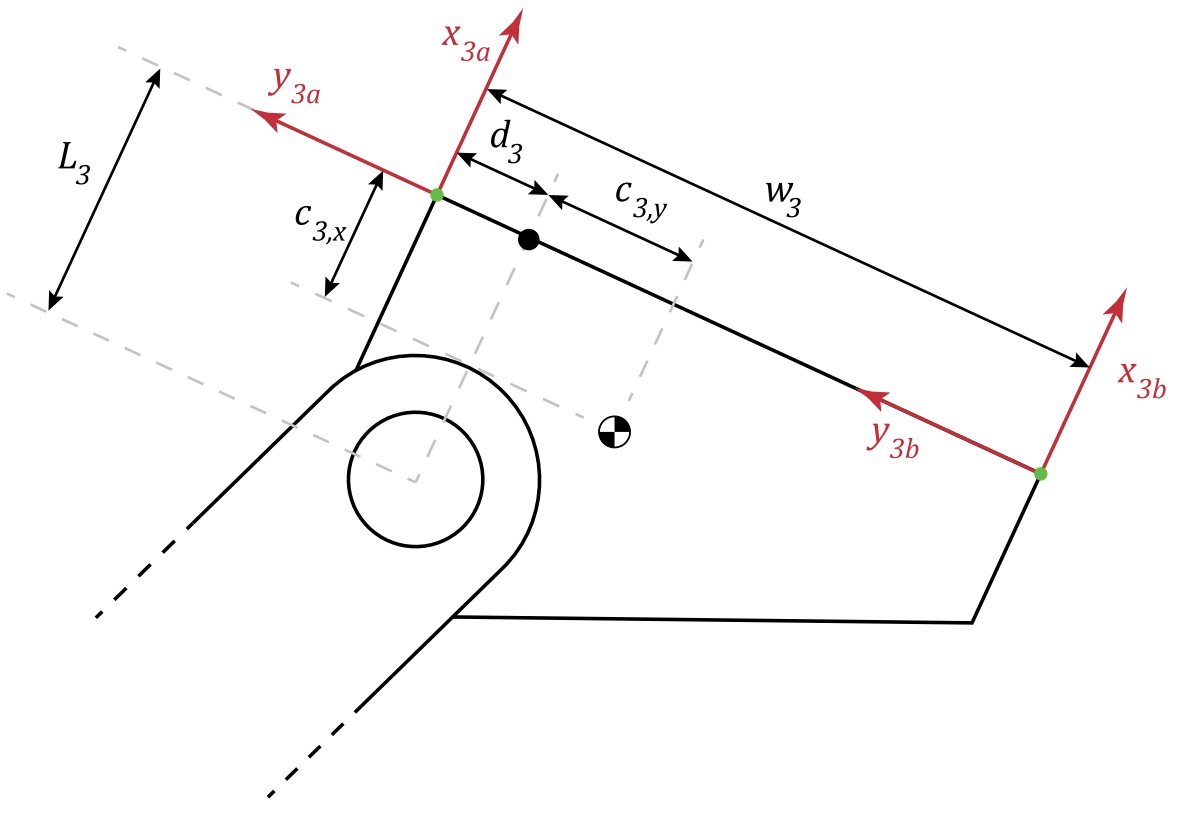
\includegraphics[width=.7\textwidth]{system2.PNG}\caption{A closer look at the foot of the RRR-robot.}
\label{fig:5system2}
\end{figure}

The generalized coordinates are defined as 
\begin{align}
\qb := \begin{bmatrix}
q_1\\q_2\\q_3\\q_4
\end{bmatrix},
\end{align}
where $\qb_i$ is the angular displacement related to the $i$-th link, as illustrated in Figure~\ref{fig:5system1}. The state of the system is then defined as
\begin{align}
\xb := \begin{bmatrix}
\qb\\\dot{\qb}
\end{bmatrix}.
\end{align}
The forward kinematics of the system are now described using homogeneous transformation matrices $\Hb^a_b$, where $\Hb^a_b$ relates coordinate frame $\Psi_b$ to coordinate frame $\Psi_a$. Since the system is in a planar setting, the transformation matrices are in the Special Euclidean group SE(2), i.e., $\Hb^a_b\in \textnormal{SE}(2)$. The transformation matrices that relate all coordinate frames to coordinate frame $\Psi_0$ are given by

\begin{align}
\Hb^0_1 &= \begin{bmatrix}
\cos(q_1) & -\sin(q_1) & L_1\cos(q_1) \\
\sin(q_1) & \cos(q_1) & L_1\sin(q_1)\\
0 & 0 & 1
\end{bmatrix},\label{eq:H01}\\
\Hb^0_2 &= \begin{bmatrix}
\cos(q_1+q_2) & -\sin(q_1+q_2) & L_1\cos(q_1) + L_2\cos(q_1+q_2) \\
-\sin(q_1+q_2) & \cos(q_1+q_2) & L_1\sin(q_1) + L_2\sin(q_1+q_2)\\
0 & 0 & 1 
\end{bmatrix},\label{eq:H02}\\
\Hb^0_3 &= \begin{bmatrix}
\cos(q_1+q_2+q_3) & -\sin(q_1+q_2+q_3) & L_1\cos(q_1) + L_2\cos(q_1+q_2) + L_3\cos(q_1+q_2+q_3) \\
-\sin(q_1+q_2+q_3) & \cos(q_1+q_2+q_3) & L_1\sin(q_1) + L_2\sin(q_1+q_2) + L_3\sin(q_1+q_2+q_3)\\
0 & 0 & 1 
\end{bmatrix},\label{eq:H03}\\
\Hb^0_4 &= \begin{bmatrix}
\cos(q_4) & -\sin(q_4) & -\Delta x \\
\sin(q_4) & \cos(q_4) & \Delta y\\
0 & 0 & 1
\end{bmatrix},\label{eq:H04}\\
\Hb^3_{3a} &= \begin{bmatrix}
1 & 0 & 0 \\
0 & 1 & d_3\\
0 & 0 & 1
\end{bmatrix},\label{eq:H33a}\\
\Hb^3_{3b} &= \begin{bmatrix}
1 & 0 & 0 \\
0 & 1 & -w_3 + d_3\\
0 & 0 & 1
\end{bmatrix}.\label{eq:H33b}
\end{align}
We now denote $x$ and $y$ the coordinates of frame $\Psi_3$ with respect to frame $\Psi_0$ in $x_0$ and $y_0$ direction respectively. We denote $\theta$ the rotation of $\Psi_3$ with respect to frame $\Psi_0$, where a positive rotation is in counterclockwise direction. The configuration of the end effector, i.e. of frame $\Psi_3$, can be obtained from \eqref{eq:H03} as
\begin{align}
\Yb:=\begin{bmatrix}
x\\y\\ \theta
\end{bmatrix} = \begin{bmatrix}
L_1\cos(q_1) + L_2\cos(q_1+q_2) + L_3\cos(q_1+q_2+q_3)\\
L_1\sin(q_1) + L_2\sin(q_1+q_2) + L_3\sin(q_1+q_2+q_3)\\
q_1+q_2+q_3
\end{bmatrix}.\label{eq:Y}
\end{align}
\nomenclature[RY]{$\Yb$}{End effector configuration}%
Since we will be considering a trajectory where the end effector makes impact with the door, the guard function associated with a open-to-closed transition, presented in Section~\ref{sec:2event}, should be evaluated. Therefore, the guard functions corresponding with contact point 1 and 2 are given by
\begin{align}
\gamma^{01} &= \hrm_{n,1}(\qb) = \begin{bmatrix} 0 & -1 & 0\end{bmatrix}\Hb^4_0\Hb^0_3\Hb^3_{3a}\begin{bmatrix}0\\0\\1\end{bmatrix}-\frac{1}{2}w_4,\\
\begin{split}
&= \Delta x\sin(q_4) + \Delta y\cos(q_4) - L_1\sin(q_1-q_4) - L_2\sin(q_1+q_2-q_4) \\
&\qquad -L_3\sin(q_1+q_2+q_3-q_4) - d_3\cos(q_1+q_2+q_3-q_4) - \frac{1}{2}w_4,
\end{split}\\
\gamma^{10} &= \hrm_{n,2}(\qb) = \begin{bmatrix} 0 & -1 & 0\end{bmatrix}\Hb^4_0\Hb^0_3\Hb^3_{3b}\begin{bmatrix}0\\0\\1\end{bmatrix}-\frac{1}{2}w_4,\\
\begin{split}
&= \Delta x\sin(q_4) + \Delta y\cos(q_4) - L_1\sin(q_1-q_4) - L_2\sin(q_1+q_2-q_4) \\
&\qquad -L_3\sin(q_1+q_2+q_3-q_4) - d_3\cos(q_1+q_2+q_3-q_4) + w_3\cos(q_1+q_2+q_3-q_4) \\ &\qquad-\frac{1}{2}w_4,
\end{split}
\end{align}
respectively. These contact distances are illustrated in Figure~\ref{fig:5guards}.
\begin{figure}[bt!]
\centering
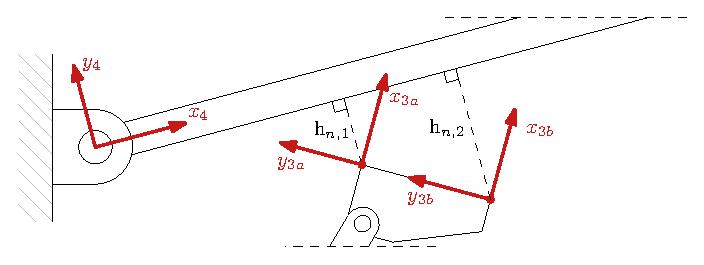
\includegraphics[width=.7\textwidth]{guards.eps}\caption{The contact distances $\hrm_{n,1}$ and $\hrm_{n,2}$ related to contact point 1 and 2.}\label{fig:5guards}
\end{figure}

\subsection{Equations of motion}
The equations of motion of the system are now presented. Since this chapter is work in progress, the system is modeled without friction. The unilateral constraints are modeled as bilateral for simplicity, and are checked for feasibility during simulation. With $\nub := \qb$ almost everywhere, the continuous dynamics of the system are given by
\begin{align}
&\Mb(\qb)\dot{\nub} + \Cb(\qb,\nub) = \Sb\ub + \sum_{\iota\in\Ic_{\text{cl}}}\wb_{n,\iota}(\qb)\lambda_{n,\iota}, &\forall \iota\in\Ic, \label{eq:5ncpcontact1}\\
&0\leq \hrm_{n,\iota}\ \bot\ \lambda_{n,\iota} \geq 0,\label{eq:5ncpcontact2}
\end{align}
with 
\begin{align}
&\hrm_{n,\iota} := \hrm_{n,\iota}(\qb),\label{eq:5h}
\end{align}
The discrete dynamics are given by
\begin{align}
&\Mb(\qb)(\nub^+ - \nub^-) = \sum_{\iota\in\Ic_{\text{cl}}} \wb_{n,\iota}(\qb)\Lambda_{n,\iota} + \Wb_{t,\iota}(\qb)\Lambdab_{t,\iota}, \label{eq:5ncpimpact1}\\
&0\leq \vrm_{n,\iota}^+\ \bot\ \Lambda_{n,\iota} \geq 0, &\forall \iota\in\Ic_{\text{cl}},\label{eq:5ncpimpact2}
\end{align}
with 
\begin{align}
\vrm^+_{n,\iota}(\qb) &:= \wb^T_{n,\iota}(\qb) \nub^+.
\end{align}
The mass matrix $\Mb(\qb)$ is given by
\begin{align}
\Mb = \begin{bmatrix}
M_{11} & M_{12} & M_{13} & 0\\
M_{12} & M_{22} & M_{23} & 0\\
M_{13} & M_{23} & M_{33} & 0\\
0 & 0 & 0 & \overline{I}_4
\end{bmatrix},
\end{align}
with
\begin{align*}
\begin{split}
M_{11} &= \bar{I}_1 +\bar{I}_2 +\bar{I}_3 + 2L_1(L_3 - c_{3,x})m_3\cos(q_2+q_3) +2L_1 c_{3,y}m_3\sin(q_2+q_3) + L_1L_2(m_2+2m_3)\cos(q_2) \\ 
&\quad+2L_2(L_3-c_{3,x})m_3\cos(q_3) + 2L_2c_{3,y}m_3\sin(q_3),
\end{split}\\
\begin{split}
M_{12} &= \bar{I}_2 + \bar{I}_3 + L_1(L_3 - c_{3,x})m_3\cos(q_2+q_3) + L_1 c_{3,y}m_3\sin(q_2+q_3) + \frac{1}{2}L_1L_2(m_2+2m_3)\cos(q_2)\\
&\quad+ 2L_2(L_3-c_{3,x})m_3\cos(q_3) + 2L_2c_{3,y}m_3\sin(q_3)
\end{split}\\
\begin{split}
M_{13} &= \bar{I}_3 + L_1(L_3 - c_{3,x})m_3\cos(q_2+q_3) + L_1 c_{3,y}m_3\sin(q_2+q_3) + L_2(L_3-c_{3,x})m_3\cos(q_3)\\
&\quad+ L_2c_{3,y}m_3\sin(q_3),
\end{split}\\
M_{22} &= \bar{I}_2 + \bar{I}_3 + 2L_2(L_3-c_{3,x})m_3\cos(q_3) + 2L_2c_{3,y}m_3\sin(q_3),\\
M_{23} &= \bar{I}_3 + L_2(L_3-c_{3,x})m_3\cos(q_3) + L_2c_{3,y}m_3\sin(q_3),\\
M_{33} &= \bar{I}_3,\\
\bar{I}_1 &= I_1 + (\frac{1}{4}m_1 + m_2 + m_3)L_1^2,\\
\bar{I}_2 &= I_2 + (\frac{1}{4}m_2 + m_3)L_2^2,\\
\bar{I}_3 &= I_3 + m_3\left((L_3-c_{3,x})^2 + c_{3,y}^2\right),
\end{align*}
where $m_1$, $m_2$, $m_3$ are the masses of link 1 to 3, and $I_1$, $I_2$, $I_3$ are the mass moment of inertia of link 1 to 3. The spring forces, damper forces, and centripetal forces form the generalized forces vector, which is given by
\begin{align}
\Cb = \begin{bmatrix}
C_1\\C_2\\C_3\\C_4
\end{bmatrix},
\end{align}
with
\begin{align*}
\begin{split}
C_1 &=-\frac{1}{2}L_1L_2(m_2+2m_3)\left(\dot{q}_2^2 + 2\dot{q}_1\dot{q}_2\right)\sin(q_2) +L_1e(q_2+q_3)\left((\dot{q}_1 + \dot{q}_2 + \dot{q}_2)^2 - \dot{q}_1^2\right)\\ 
&\qquad+ L_2e(q_3)\left(\dot{q}_3^2 + 2\dot{q}_1\dot{q}_3 + 2\dot{q}_2\dot{q}_3\right),
\end{split}\\
C_2 &= \frac{1}{2}L_1L_2(m_2+2m_3)\sin(q_2) - L_1e(q_2+q_3)\dot{q}_1^2 + L_2e(q_3)\left(\dot{q}_3^2 + 2\dot{q}_1\dot{q}_3 + 2\dot{q}_2\dot{q}_3\right),\\
C_3 &= -L_1e(q_2+q_3)\dot{q}_1^2 - L_2e(q_3)(\dot{q}_1+\dot{q}_2)^2,\\
C_4 &= c_d\dot{q}_4 + c_k q_4,
\end{align*}
where
\begin{align*}
e(q) = m_3\left(c_{3,y}\cos(q) - (L_3-c_{3,x})\sin(q)\right).
\end{align*}
The selection matrix is $\Sb = \begin{bmatrix}\Ib_3 & \Zerob_{3 \times 1}\end{bmatrix}$. Finally, the jacobians $\wb_{n,1}^T$ and $\wb_{n,2}^T$ are defined by $\dot{\hrm}_{n,1} = \wb_{n,1}^T \dot{\qb}$ and $\dot{\hrm}_{n,2} = \wb_{n,2}^T \dot{\qb}$, which give
\begin{align}
\wb_{n,1} &= \begin{bmatrix}
a(\qb) + b(\qb) + c(\qb) + d(\qb)\\
b(\qb) + c(\qb) + d(\qb)\\
c(\qb) + d(\qb)\\
-a(\qb) - b(\qb) - c(\qb) - d(\qb) + \Delta x\cos(q_4) - \Delta y\sin(q_4)
\end{bmatrix},\\
\wb_{n,2} &= \begin{bmatrix}
a(\qb) + b(\qb) + c(\qb) + d(\qb)-w_3\sin(q_1+q_2+q_3-q_4)\\
b(\qb) + c(\qb) + d(\qb)-w_3\sin(q_1+q_2+q_3-q_4)\\
c(\qb) + d(\qb)-w_3\sin(q_1+q_2+q_3-q_4)\\
-a(\qb) - b(\qb) - c(\qb) - d(\qb) + \Delta x\cos(q_4) - \Delta y\sin(q_4)+w_3\sin(q_1+q_2+q_3-q_4)
\end{bmatrix},
\end{align}
with
\begin{align*}
a(\qb) &= -L_1\cos(q_1-q_4),\\
b(\qb) &= -L_2\cos(q_1+q_2-q_4),\\
c(\qb) &= -L_3\cos(q_1+q_2+q_3-q_4),\\
d(\qb) &= d_3\sin(q_1+q_2+q_3-q_4).
\end{align*}
The kinematics presented in Section~\ref{sec:5kin} and the dynamics presented in this section are first derived in \cite{Rijnen2018b}. For a more thorough derivation of the kinematics and dynamics, the reader is referred to that work. In the next section a tracking simulation for the example system is simulated and discussed. 
\section{Trajectory tracking with simultaneous impact}\label{sec:5track}
Using the system presented in Section~\ref{sec:5sys}, the results of the trajectory tracking simulation will be discussed in this section. The considered reference trajectory contains a simultaneous impact between the two contact points and the door. First, the design of the reference trajectory will be discussed, where the resulting reference trajectory satisfies the assumptions posed in this work. Then, the simulation results are presented. Here the tracking behavior around the reference trajectory with simultaneous impacts is discussed, and the benefits of the reference spreading error are illustrated. The simulations presented in this section are performed using MATLAB and a hybrid systems toolbox written by the author of \cite{Rijnen2018a}.

\subsection{Reference trajectory design}
To design the reference trajectory, a Hermite interpolation is used to interpolate between the desired initial state and input and the desired final state and input. The Hermite interpolation makes use of the quintic polynomial functions
\begin{align}
y(t) &=  a_0 + a_1t + a_2t^2 + a_3t^3 + a^4t^4 + a_5t^5,\\
\dot{y}(t) &= a_1 + 2a_2t + 3a_3t^2 + 4a^4t^3 + 5a_5t^4,\\
\ddot{y}(t) &= 2a_2 + 6a_3t + 12a^4t^2 + 20a_5t^3,
\end{align}
where the coefficients of the polynomial $a_0$ to $a_5$ are determined by the system
\begin{align}
\begin{bmatrix} 1 & t_{0} & t_0^2 & t_0^3 & t_0^4 & t_0^5\\
 0 & 1 & 2\,t_{0} & 3\,t_0^2 & 4\,t_0^3 & 5\,t_0^4\\
 0 & 0 & 2 & 6\,t_{0} & 12\,t_0^2 & 20\,t_0^3\\
 1 & t_f & t_f^2 & t_f^3 & t_f^4 & t_f^5\\
 0 & 1 & 2\,t_f & 3\,t_f^2 & 4\,t_f^3 & 5\,t_f^4\\
 0 & 0 & 2 & 6\,t_f & 12\,t_f^2 & 20\,t_f^3 \end{bmatrix}\begin{bmatrix}
a_0\\a_1\\a_2\\a_3\\a_4\\a_5
\end{bmatrix}
= \begin{bmatrix}
y_0\\ \dot{y}_0\\ \ddot{y}_0\\y_f\\ \dot{y}_f\\ \ddot{y}_f
\end{bmatrix}.\label{eq:5hermite}
\end{align}
Here $t_0$ and $t_f$ are the start- and end-time of the trajectory segment, respectively, $y_0$, $\dot{y}_0$, and $\ddot{y}_0$ the position, velocity and acceleration at the start of the trajectory segment, and $y_f$, $\dot{y}_f$, and $\ddot{y}_f$ the position, velocity and acceleration at the end of the trajectory segment.

The Hermite interpolation is now used to define a reference trajectory. The reference is defined on task level, i.e., the configuration of the end effector $\Yb$ is prescribed. Three event times are introduced: $\tau_0$ is initial time of the reference, $\tau_1$ is the event time of the simultaneous impact, and $\tau_2 = \tau_f$ is the final time of the reference. The ante-event segment of the reference, $t \in [\tau_0,\tau_1]$, has the initial and final conditions
\begin{align}
x_0&= 0.650 &x^-_1&= 0.433 &y_0&= 0 &y^-_1&= 0.280 &\theta_0&= \pi/5 &\theta^-_1&= \pi/2\nonumber\\
\dot{x}_0&= 0 &\dot{x}^-_1&= -0.250 &\dot{y}_0&= 0 &\dot{y}^-_1&= 0.350 &\dot{\theta}_0&= 0 &\dot{\theta}^-_1&= 0\label{eq:5traj01}\\
\ddot{x}_0&= 0 &\ddot{x}^-_1&= -0.700 &\ddot{y}_0&= 0 &\ddot{y}^-_1&= 2 &\ddot{\theta}_0&= 0 &\ddot{\theta}^-_1&= 0\nonumber
\end{align}
Note that we only define the left limits for $t=t_1$, because the right limits are defined by the discrete dynamics \eqref{eq:5ncpimpact1}-\eqref{eq:5ncpimpact2}. During the design of the ante-event segment, we assume the door to be closed, i.e., $q_4=\dot{q}_4=\ddot{q}_4$ for all $t\in[\tau_0,\tau_1]$. The conditions \eqref{eq:5traj01} define the trajectory for $t\in[\tau_0,\tau_1]$ using the hermite interpolation \eqref{eq:5hermite}. This trajectory is now extended, where the final conditions of the left extension are
\begin{align}
x^-_{\textnormal{ext}}&= 0.353 &y^-_{\textnormal{ext}}&= 0.400 &\theta^-_{\textnormal{ext}}&= \pi/2\nonumber\\
\dot{x}^-_{\textnormal{ext}}&= -0.580 &\dot{y}^-_{\textnormal{ext}}&= 0.830 &\dot{\theta}^-_{\textnormal{ext}}&= 0\\
\ddot{x}^-_{\textnormal{ext}}&= -0.700 &\ddot{y}^-_{\textnormal{ext}}&= 2 &\ddot{\theta}^-_{\textnormal{ext}}&= 0\nonumber
\end{align}

These conditions result in the trajectories illustrated in Figure~\ref{fig:5traj}.
\begin{figure}[bt!]
\begin{minipage}[c]{.5\textwidth}
\centering
\caption*{ante-event reference trajectory}
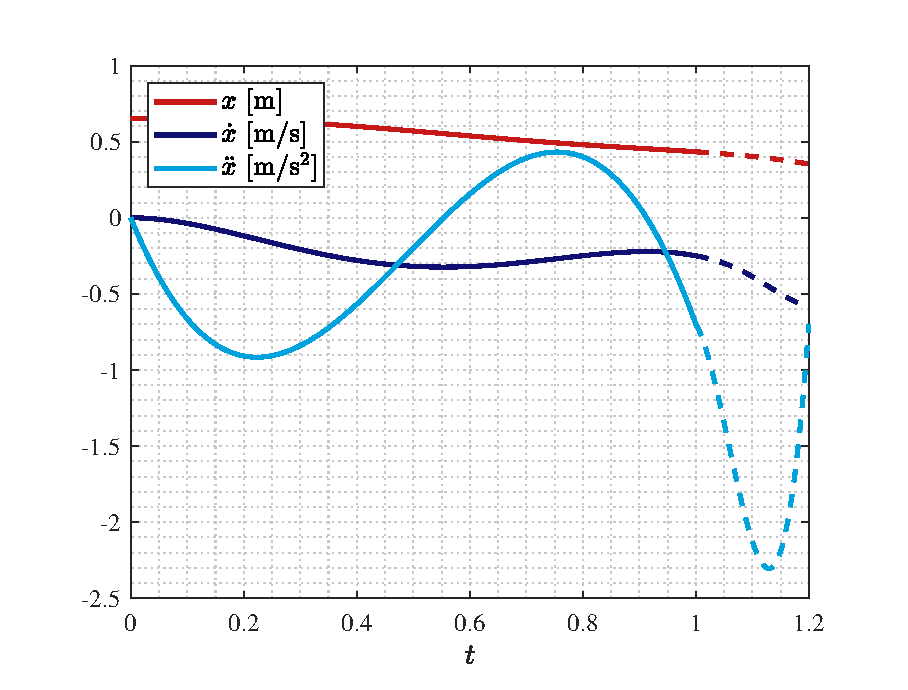
\includegraphics[width=\textwidth]{xtraj01.eps}
\end{minipage}
\begin{minipage}[c]{.5\textwidth}
\centering
\caption*{post-event reference trajectory}
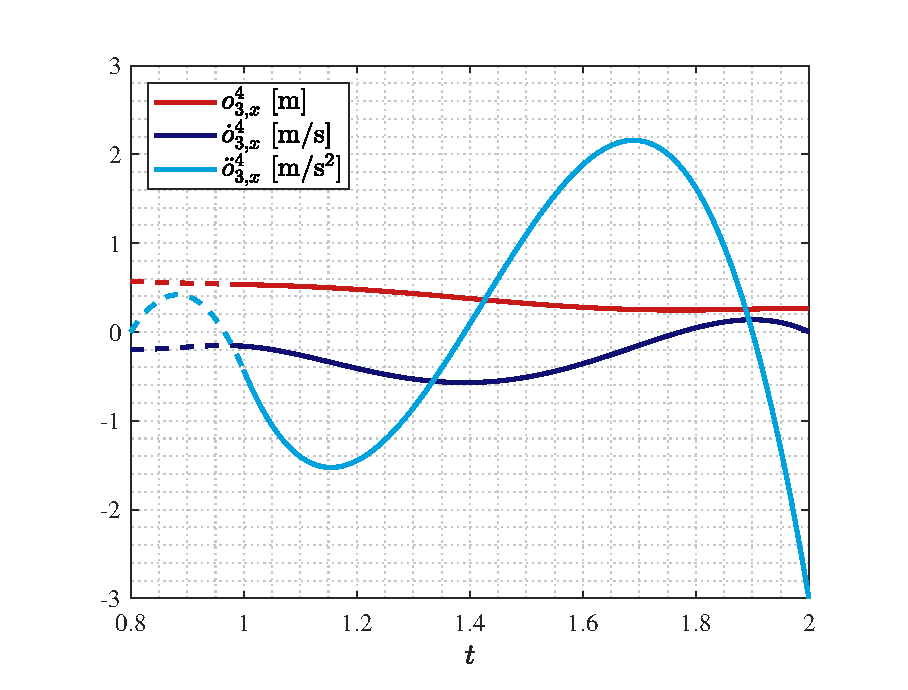
\includegraphics[width=\textwidth]{o3xtraj12.eps}
\end{minipage}

\begin{minipage}[c]{.5\textwidth}
\centering
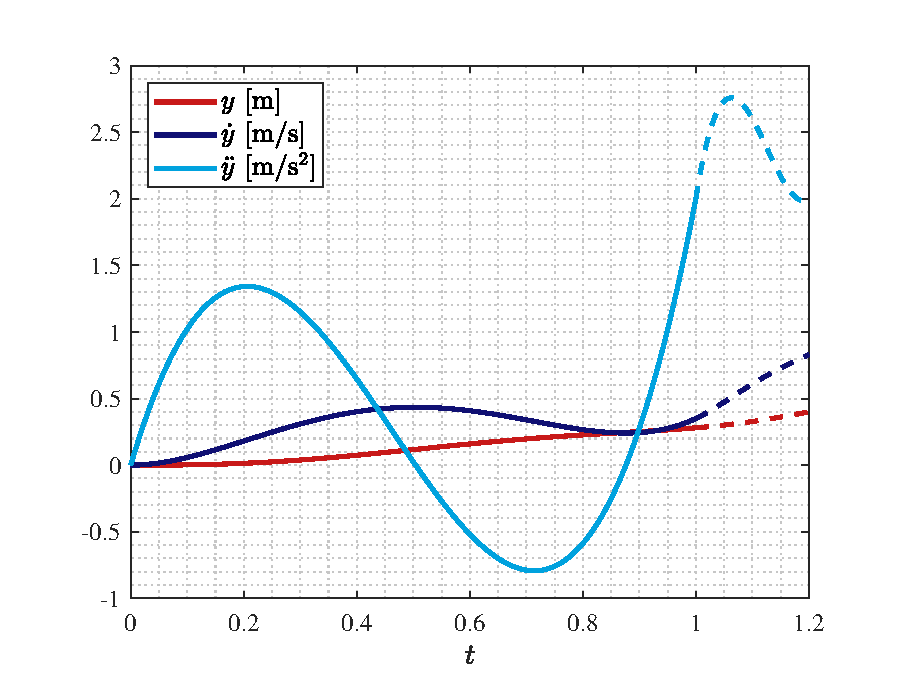
\includegraphics[width=\textwidth]{ytraj01.eps}
\end{minipage}
\begin{minipage}[c]{.5\textwidth}
\centering
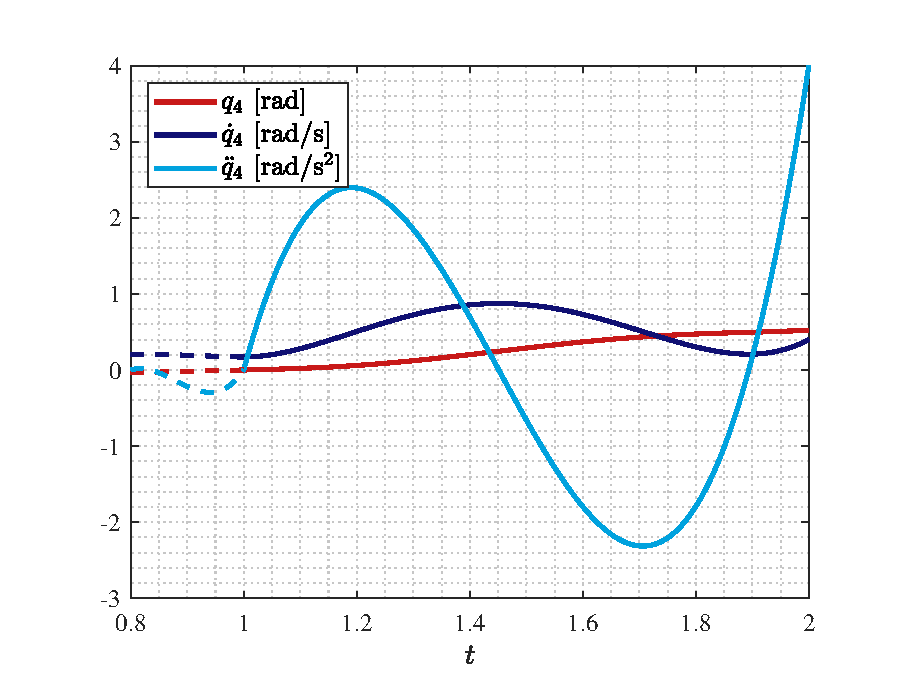
\includegraphics[width=\textwidth]{q4traj12.eps}
\end{minipage}

\begin{minipage}[l]{.5\textwidth}
\centering
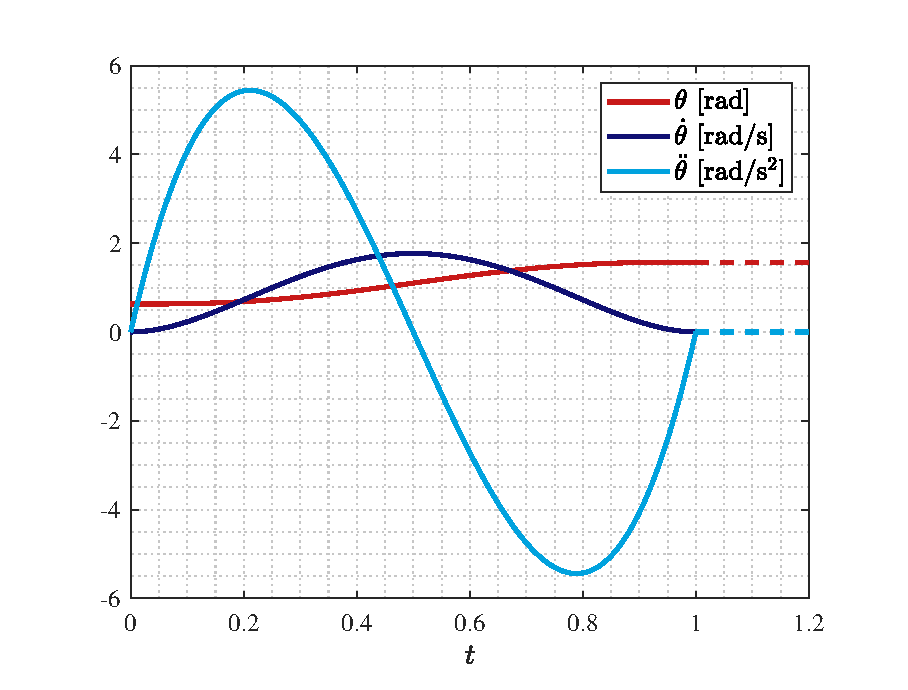
\includegraphics[width=\textwidth]{thtraj01.eps}
\end{minipage}
\caption{The reference trajectory for $t\in[\tau_0,\tau_2]$. On the left is the ante-event reference trajectory, with in the left-top image $x$, $\dot{x}$, $\ddot{x}$, the left-middle image $y$, $\dot{y}$, $\ddot{y}$, and in the left-bottom image $\theta$, $\dot{\theta}$, $\ddot{\theta}$. On the right is the post-event reference trajectory, with in the right-top image $o_{3,x}^4$, $\dot{o}_{3,x}^4$, $\ddot{o}_{3,x}^4$, and in the right-middle image $q_4$, $\dot{q}_4$, $\ddot{q}_4$. The dashed lines indicate the extensions past $\tau_1$.}
\label{fig:5traj}
\end{figure}
The post-event segment of the trajectory is now designed in a similar fashion. Since the end-effector is constrained to the door during the post-event trajectory, $\hrm_{n,1} = \hrm_{n,2} = 0$ (and their derivatives as well). Because of these constraints, a state reduction can be applied. The initial and final conditions for the post-event segment are
\begin{align}
(o_{3,x}^4)^+_{\textnormal{ext}}&= 0.650 &(o_{3,x}^4)_2&= 0.433 &(q_4)^+_{\textnormal{ext}}&= 0 &(q_4)_2&= 0.280\nonumber\\
(\dot{o}_{3,x}^4)^+_{\textnormal{ext}}&= 0 &(\dot{o}_{3,x}^4)_2&= -0.250 &(\dot{q}_4)^+_{\textnormal{ext}}&= 0 &(\dot{q}_4)_2&= 0.350 \label{eq:5traj12}\\
(\ddot{o}_{3,x}^4)^+_{\textnormal{ext}}&= 0 &(\ddot{o}_{3,x}^4)_2&= -0.700 &(\ddot{q}_4)^+_{\textnormal{ext}}&= 0 &(\ddot{q}_4)_2&= 2 \nonumber
\end{align}
where $o_{3,x}^4$ is the position of the $\Psi_3$ frame in the $x$-direction of frame $\Psi_4$, that is the position of the end effector along the door. The conditions in \eqref{eq:5traj12} are used instead of $\Yb$, for a more intuitive design process of the trajectory. The super- and subscript $(\cdot)_ext^+$ indicates the initial condition of the trajectory extension, and the subscript $(\cdot)_2$ indicates the final condition of the post-event trajectory. The post-event reference trajectory resulting from \eqref{eq:5traj12} is illustrated in Figure~\ref{fig:5traj}.

\subsection{Simulation results}
A trajectory tracking simulation is performed with the system presented in Section~\ref{sec:5sys}.
\begin{itemize}
\item nominal trajectory plot + inputs
\item tracking plot + inputs
\item \textbf{tracking error vs rs error}
\end{itemize}

\section{Future work}


\section{Summary}

\end{document}